\subsection{Solidity ABI \& Exposed Functions}
The Solidity \textit{Application Binary Interface} (short: ABI) is a convention for contract interaction which specifies the function calls between contracts on the bytecode-level. To explain to potential users how to call a contract deployed on the blockchain, a \textit{contract interface} (for example a JSON-file generated by the Solidity-compiler) can be published, which contains the signatures of the functions available in the contract.

\subsubsection{Non-Restricted Function Accessibility}
Because the contract interface is not stored on the blockchain, using the ABI correctly and only calling functions specified in the published interface is not enforced by the protocol. The contract creator has to make sure that no internal function is called. Since the Solidity compiler only generates entry points for the functions marked as public, this is usually not a problem. But if for some reason the user decides to bypass those mechanisms, this can lead to serious damage:

\paragraph{Embedding Library Functions} Since deploying complex code to the Ethereum blockchain requires gas (and therefore costs Ether) proportional to the amount of EVM bytecode deployed as a payment to the miners, it became popular to extract and store most of the code in library smart contracts like the contract in listing \ref{lst:abi:library}.

\begin{listing}[H]
	\begin{minted}[
        linenos=true,
        firstnumber=1
    ]{solidity}
contract SimpleWalletLibrary { 
    address public owner;
    function () public payable {}
    function initWallet(address _owner) public {
        owner = _owner;
    }
    function kill() public {
        require(msg.sender == owner);

        selfdestruct(owner);
    }
    // ...
}
    \end{minted}
	\caption{The library contract \texttt{SimpleWalletLibrary}}
	\label{lst:abi:library}
\end{listing}

To access the functions in the library from inside another contract, the low-level command \texttt{delegate\-call} can be used, which executes the bytecode of the library contract using the execution context (the storage of the contract, ownedEther etc.) of the caller (see section \ref{section:deepdive:evm} for more details). To invoke a specific library function, its signature hash has to be provided along with the parameters:
\begin{minted}{solidity}
simpleWalletLibrary.delegatecall(bytes4(keccak256("initWallet(address)")), owner);
\end{minted}

Because it would still require a lot of bytecode to create an explicit function executing \texttt{delegate\-call} for every function of the library code to be included, in some contracts the fallback function is used to redirect all calls whose signature hash did not match any of the regular functions inside the contract to the corresponding function of the library contract:
\begin{minted}{solidity}
function() public payable {
    simpleWalletLibrary.delegatecall(msg.data);
}
\end{minted}

Using this trick the published contract interface of the main contract is able to contain functions from the library contract, which can be called as if they were explicitly declared inside:
\begin{minted}{solidity}
contract SimpleWalletABI {
    function kill() public;
    function () public payable;
}
\end{minted}

Although in this example \mintinline{solidity}{initWallet(address)} is not explicitly mentioned in the published contract interface, it can still be used since the call will nevertheless be forwarded by the fallback function. This enables anyone to become the owner of the instance of the \texttt{Wallet} contract.

\subparagraph{Parity Wallet Stealing}
A contract using the library-pattern was the Multi-Signature Wallet the Parity client used as a template contract. A \textit{Multi-Signature Wallet} is a special contract that stores crypto-currencies for a group of people (for example the founders of a start-up) and requires the approval of several owners to make sure no one alone can steal the funds. One of the authors of the Wallet-Contract was the inventor of the Solidity-ABI, Gavin Wood.\footnote{see \cite{wikisource:solidityinventorgavinwood} for Gavin Wood being the inventor of the ABI, \cite{code:parityenhancedwalletsteal} for him writing the contract}

The vulnerability of the Wallet contract, that can be found at \cite{code:parityenhancedwalletsteal}, is the following: In the library \mintinline{solidity}{contract WalletLibrary}, there is the initializer function \mintinline{solidity}{initMultiowned(address[] _owners, uint _required)} which sets the owners of the Multi Signature Wallet without checking if they were already set. This function is called in the constructor of \texttt{Wallet} using \texttt{de\-le\-gate\-call}, but could still be accessed in the Wallet because inside the fallback function \mintinline{solidity}{function() payable} every call with an unmatched function selector gets forwarded to the \texttt{WalletLibrary}.

Because of this, the attacker just had to call \mintinline{solidity}{initMultiowned(["0x<ownAddress>"], 0)} on a wallet to set themself as the owner and disable the requirement of multiple approvals; and afterwards use its \texttt{execute}-function to transfer its contents to another account.\footnote{see \cite{etheraveum:paritywallethackexplained}. The function calls were done in the transactions \cite{etherscan:walletsteal:inittransaction} and \cite{etherscan:walletsteal:executetransaction}.}

The attack took place on 19th of July 2017 and emptied three MultiSignature-Wallets obtaining about 30 million US-\$ in Ether at that time. Soon a group of \textit{white-hat hackers} (hackers using their knowledge to help the public) had noticed and analyzed the attack and started exploiting the vulnerability as well as trying to rescue the Ether out of the vulnerable wallets. If the attacker would have had more time, they could have stolen up to additional 90 million US-\$ of Ether. (see \cite{freecodecamp:paritywallethackexplained}) Until time of writing, the attacker has not retrieved their yield, probably to keep their identity concealed.\footnote{see the account balance of the hacker at \cite{etherscan:walletsteal:account}}. This bug was fixed by Parity by adding a modifier \mintinline{solidity}{only_uninitialized()} to the initializer-functions, which prevents the function from being called when the owners have already been set.

\subsubsection{Libraries Called in their own Context}
Listing \ref{lst:abi:library} contains another vulnerability: While only intended to be used as a library and not called directly, the deployed \mintinline{solidity}{WalletLibrary} has some of the functionality of a regular \mintinline{solidity}{Wallet} when called directly (and therefore is working in its own context). This includes becoming the owner of the contract by using \mintinline{solidity}{initWallet("0x<ownAddress>")} and then deleting the contract using \mintinline{solidity}{kill()}.

This "suicide" of the library will remove the library code from the blockchain state thus rendering all contracts calling the library useless, since now all the calls to that contract will just return \mintinline{solidity}{false}.

A possible solution to this problem is using the contract type \mintinline{solidity}{library}, which will make the compiler add a check whether the address of the execution context is equal to the address of the context used when deploying the contract, and if so, revert the execution.

\paragraph{Parity Library Suicide}
As a response to the first attack against the wallets a fixed version of the \texttt{WalletLibrary} was deployed, which was then used starting from 20th of July 2017 as the new template contract in the Parity Client. But while the initialization function was secured, this vulnerability was overlooked:

On  the 6th of November 2017 someone sent a call to \mintinline{solidity}{initMultiowned(["0x<ownAddress>"], 0)} to become the "owner" of the \mintinline{solidity}{WalletLibrary}, followed by \mintinline{solidity}{kill("0x<ownAddress>")}.\footnote{as done by the attacker in \cite{etherscan:walletfreeze:init} and \cite{etherscan:walletfreeze:kill}}

This rendered more than half a million Ether (at the time of the attack about 150 million US-\$\footnote{at 296.43 US-\$ / Ether, the opening price of November, the 6th 2017; according to \cite{coinmarketcap:parityfreeze}}) that had been stored in 587 different MultiSignature-Wallets inaccessible. (see \cite{parity:postmortem}) After the attack, a GitHub-User called \texttt{devops199} claimed to be the owner of the address that launched the attack -- and that they did not know what they were doing.\footnote{see \cite{springrole:parityfreeze}; the issue is located at \cite{github:devops199}}

After the attack, some people affected by the bug demanded a change in the protocol, a so-called \textit{fork}. If only a part of the miners implements those changes, the blocks produced by miners running different protocol versions could become incompatible and therefore the blockchain would split.

In the case of Ethereum and the Parity Library Freeze, the change could restore a fixed version of the library at its old address to make the frozen wallets accessible again. In Ethereum Improvement Proposal 999 this idea was formally proposed by Parity employee Afri Schoedon, which has not been accepted and implemented up to now.\footnote{located at \cite{github:eic999}}

One argument against the fork was, that if not every participant agreed, another alternative blockchain would be created. Additionally, many users felt like the vulnerability could have been prevented by an audit and better security measurements, especially because this bug had already been known back in August 2017, three months before the attack -- it was recommended to claim ownership of the library when deploying by GitHub-user \texttt{3esmit} in a pull-request on the Parity Contract-Repository.\footnote{can be found at \cite{github:parityinitialize}} As a reaction to that attack Parity announced in a blog post that they are planning to reduce their own smart contract development, they were planning to use better tooling to detect vulnerabilities and that they had partnered with an auditing company to validate their smart contracts. (see \cite{parity:newdevprocesses})

\subsubsection{Constructors of Renamed Contracts}
When a smart contract is being created, the code inside the constructor, a function with the same name as the contract, is executed. Afterwards, this code is not inside of the deployed contract bytecode and therefore can't be called again. Usually the constructor is used to initialize the smart contract, for example by giving the contract's creator special privileges.

\begin{listing}[H]
	\begin{minted}[
        linenos=true,
        firstnumber=1
    ]{solidity}
contract NewContractName {
    address owner;
    function OldContractName() public {
        owner = msg.sender;
    }
    // ...
}
    \end{minted}
	\caption{The smart contract \texttt{OldContractName} was renamed to \texttt{NewContractName} without updating the constructor name.}
	\label{lst:abi:newcontractname}
\end{listing}

If the contract is renamed afterwards without changing the name of the constructor function, the constructor becomes a regular function -- and is invocable by anyone. In the case of \mintinline{solidity}{NewContractName} in figure \ref{lst:abi:newcontractname}, now everyone can call the constructor at any time and therefore become the owner of the smart contract.

Starting with Solidity v0.4.22 released in April 2018, the new default constructor syntax is \mintinline{solidity}{constructor ()} instead of \mintinline{solidity}{function OldContractName()}, which does not have to be modified when changing the contract name.\footnote{see solidity changelog at \cite{solidity:changelog}}

\paragraph{Rubixi-Ponzi}
Ponzi schemes are a fraudulent investment scheme, where the payout to prior investors is paid using the money of new participants. Some owners impose a fee on the participants, that can be later retrieved by the owner using a contract function. (see \cite[section 4.4]{atzei:attacksurvey})

One of those schemes was the \texttt{Rubixi}-Ponzi, whose owner had changed the name from \texttt{Dynamic\-Py\-ra\-mid} without updating the constructor name. Due to this everyone was able to retrieve the collected fees using \mintinline{solidity}{collectAllFees()} after becoming the owner by calling the unprotected constructor.\footnote{the smart contract code can be found at \cite{etherscan:rubixi}}

\subsubsection{Wrong Interfaces}
Another possible vulnerability of smart contracts is using them with contract interfaces that are different from the one generated from the contract code:

Since the interface and source code of a smart contract is not stored on the blockchain, other ways have to be used to get the information necessary to interact with a contract. One way are pages like \url{etherscan.io} that can be used to publish the contract source-code for contracts that are already on the blockchain, and even validates that the deployed contract has a bytecode that was compiled from the given source code. But this only works for around 1 \% of the contracts that provide their bytecode on Etherscan.\footnote{calculated by \cite[Introduction]{nikolic:findingbadcontractsatscale}}

Because of this, users will most of the time have to get the contract interface from other, inverified sources or reverse-engineering of the bytecode. In the following I will present some ways on how this could be exploited:

\paragraph{Fallback Function because of Wrong Interface}
In the most probable case a contract is called with a function selector hash that does not correspond to any of the declared functions: In that case, the fallback function will handle this request, that may make the execution of the command fail, or even lead to unwanted behavior:

The following bank-contract stores the balance of each user in a \mintinline{solidity}{mapping} and allows donating Ether to the owner by using the fallback function:
\begin{minted}{solidity}
contract Bank {
    // ...
    // tip to owner
    function () public payable {
        deposit(owner);
    }
    function deposit(address user) public payable {
        balance[user] += msg.value;
    }
}
\end{minted}

When writing a smart contract interacting with this bank contract (or when using a wallet application) the contract interface has to be entered, which might include mistakes like typing errors:
\begin{minted}{solidity}
contract BankABI { function deopsit(address user) public payable; }
\end{minted}

Since \mintinline{solidity}{deopsit(address)} has a signature hash of \texttt{425f42f2}, it won't match the hash of the function \mintinline{solidity}{deposit(address)} (which is \texttt{f340fa01}), so that the fallback function gets executed. Because of this, the received Ether will be added to the account of the owner instead of the one specified by the user.\footnote{a similar idea is presented in \cite[wrong\_interface]{trailofbits:notsosmartcontracts}}

\paragraph{Using Selector Collision to Trick Users}
Another possible way to attack a smart contract is to deceive its users into calling contracts with inputs that are malicious to them. This could be done by providing a faked source code, that makes the user call the contract with special inputs:

In this example, the user is owner of some tokens managed by the smart contract \texttt{BuckToken}, that contains the following function:
\begin{minted}{solidity}
function sendThoseBucksToTheAccountThanks(uint amount, bool createLog, address to) public
\end{minted}

To steal tokens from the user, the attacker presents the bounty contract and claims that the contract is located at the address of the \texttt{BuckToken}.

\begin{minted}{solidity}
contract BountyContract {
    function () public payable {}
    function compareParametersAndRecieveCryptoInstantaneously(int[] attempt) public {
        require(attempt.length == 1);
        require(attempt[0] == 1154414090619811796818182302139415280051214250812);
        msg.sender.transfer(1 Ether);
    }
}
\end{minted}

Because the bounty contract releases the money only for a special input, the user might try to send the input deduced from the code to the function:
\begin{minted}{solidity}
compareParametersAndRecieveCryptoInstantaneously([
    1154414090619811796818182302139415280051214250812
])
\end{minted}

Since the selector hashes of \mintinline{solidity}{compareParametersAndRecieveCryptoInstantaneously(int256[])} and \mintinline{solidity}{sendThoseBucksToTheAccountThanks(uint256,bool,address)} are both equal to \texttt{a09abf73}, the contract recognizes this as a call to \texttt{send\-Those\-Bucks\-To\-The\-Account\-Thanks} and decodes the arguments in a different way (see figure \ref{fig:payloadlayout}) -- which will move \( 20 \) tokens from the account holder to the specified address:
\begin{minted}{solidity}
sendThoseBucksToTheAccountThanks(20, true, "0xca35b7d915458ef540ade6068dfe2f44e8fa733c")
\end{minted}

\vspace{1em}
\begin{minipage}{\linewidth}
	\centering
	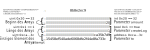
\includegraphics[scale=1.0]{img/abi/calldatalayout.pdf}
	\captionof{figure}[Payload Layout]{The payload of the function calls \texttt{compareParametersAndRecieveCrypto\-In\-stan\-taneous\-ly(32, true, 0xca...3c)} and \texttt{checkSecretAndGetWeiKindly([11...12])} is identical.}
	\label{fig:payloadlayout}
\end{minipage}

If the user does not recognize the Token contract from the address they are interacting with, because of the different function name and the completely different parameters, they won't be reminded of the former interaction with the first contract.

To obtain function signatures with the same hashes, \textsc{Sact}, a simple program (presented in appendix \ref{appendix:abicollision}) was written to find them using brute force. To speed up calculations and reduce the amount of different selectors to try (to get prettier names), the collision tests were run against a dictionary of possible selectors, so that finding a collision was possible using a single thread within a few seconds. In the example of the next paragraph, the collision tests were run against a single selector, which requires an expected amount of around four billion hashing operations. To find those collisions, it took around 15 minutes using four parallel threads.

\paragraph{Obfuscation of Malicious Contracts}
Another way to abuse function selector collisions could be obfuscation of malicious code. For example when writing an exploit for the following \texttt{Wallet}, it might be of interest to hide that the code is interacting with this specific contract interface.

To achieve this, colliding function selectors can be calculated and used instead of original selectors. Since additional parameters are ignored by the contract bytecode generated by Solidity, random additional parameters can be added for additional confusion. The functions of the following contract interfaces have identical function selectors hashes for each line:

\begin{multicols}{2}
	\begin{minted}{solidity}
contract Wallet {
    function deposit() payable;
    function withdraw();
}
\end{minted}

	\begin{minted}{solidity}
contract WeirdContractInterface {
    function wFyuDA(string a) payable;
    function EcctzE(
        uint256 a, address b);
}
\end{minted}
\end{multicols}
